\section{Introduction}

\subsection{Run-Through}
\begin{frame}
\frametitle{Compact Run-Through}
	\begin{figure}
		\centering
		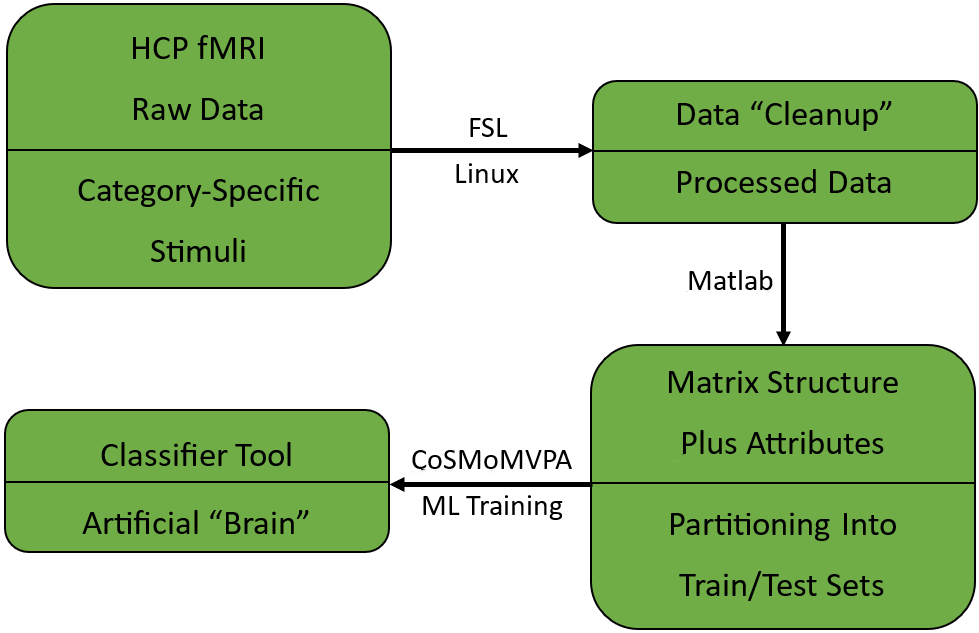
\includegraphics[width=\textwidth]{assets/jist.png}
	\end{figure}
\end{frame}


\subsection{Decoding and Classification}
\begin{frame}
\frametitle{Decoding}

    \begin{itemize}
        \uncover<1->{\item To connect neural patterns with specific human functions}
        \uncover<2->{\item From brain activation to identifying object of perception}
        \uncover<3->{\item Certain areas are linked to category-specific stimuli processing}
        \uncover<4->{\item Assessment of baseline BOLD signal magnitude (\textit{UPA})}
        \uncover<5->{\item Comparison of pattern distributions (\textit{MVPA})}
    \end{itemize}
\end{frame}

\begin{frame}
\frametitle{Classification}
	\begin{columns}
		\begin{column}{0.5\textwidth}
			\begin{itemize}
				\uncover<1->{\item Supervised Machine Learning}
				\uncover<2->{\item Train model on labeled data,\\predict labels of test data}
				\uncover<3->{\item Support Vector Machine algorithm to determine boundaries}
			\end{itemize}
		\end{column}

		\begin{column}{0.49\textwidth}
			\only<2>{
				\begin{figure}
					\centering
					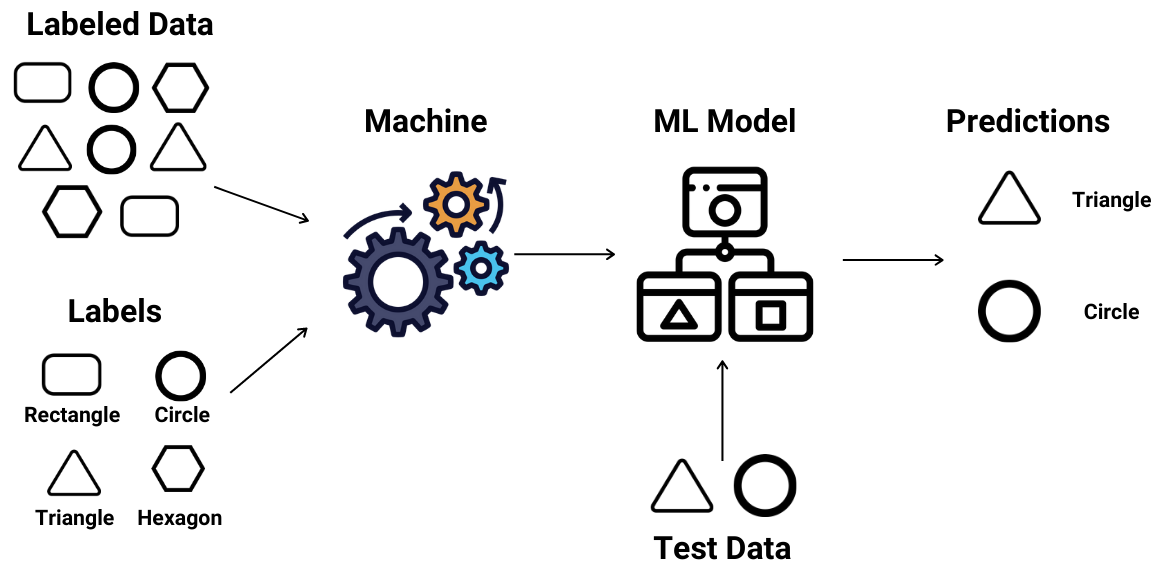
\includegraphics[width=\textwidth]{assets/class.png}
				\end{figure}
				}
			\only<3>{
				\begin{figure}
					\centering
					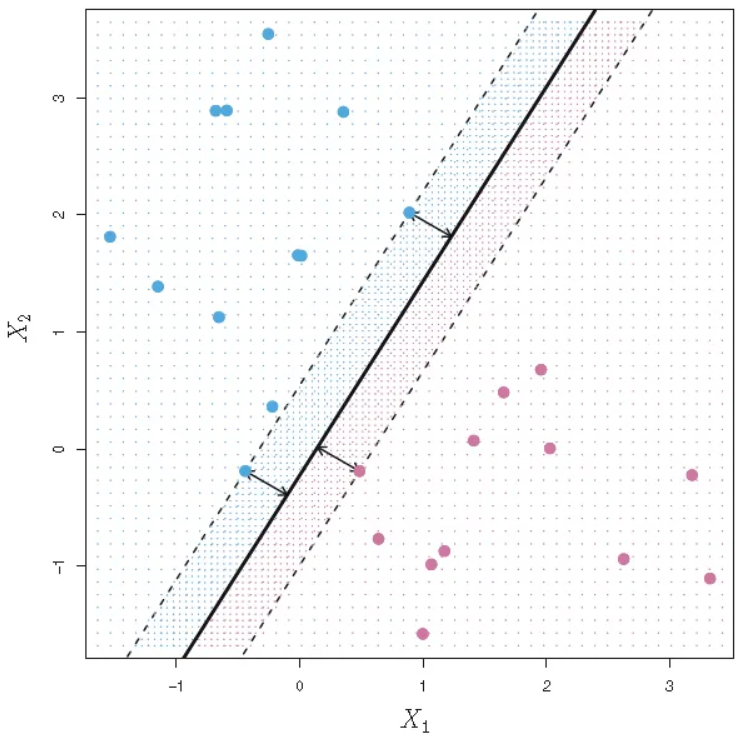
\includegraphics[width=\textwidth]{assets/svm_simple.png}
					\caption*{\ \ \ \ \ SVM - Linear Separation}
				\end{figure}
				}
		\end{column}
	\end{columns}	
\end{frame}

\begin{frame}
\frametitle{SVM - Linear Separation - Kernel Trick}
	\begin{figure}
		\centering
		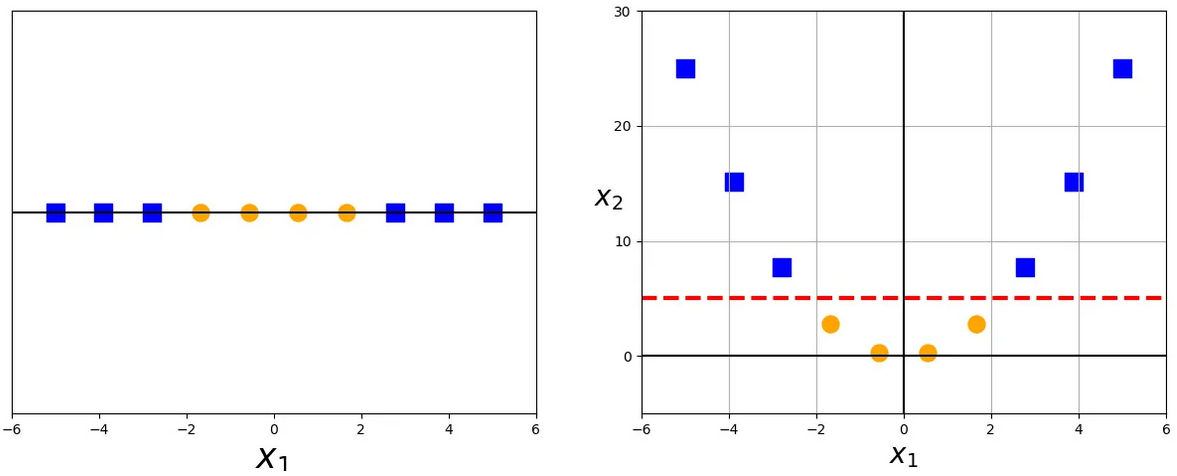
\includegraphics[width=0.98\textwidth]{assets/svm_comp_1.png}
		\caption*{SVM - Linear Separation - Kernel Trick}
	\end{figure}
\end{frame}

\begin{frame}
\frametitle{SVM - Non-Linear Separation - Kernel Trick}
	\begin{figure}
		\centering
		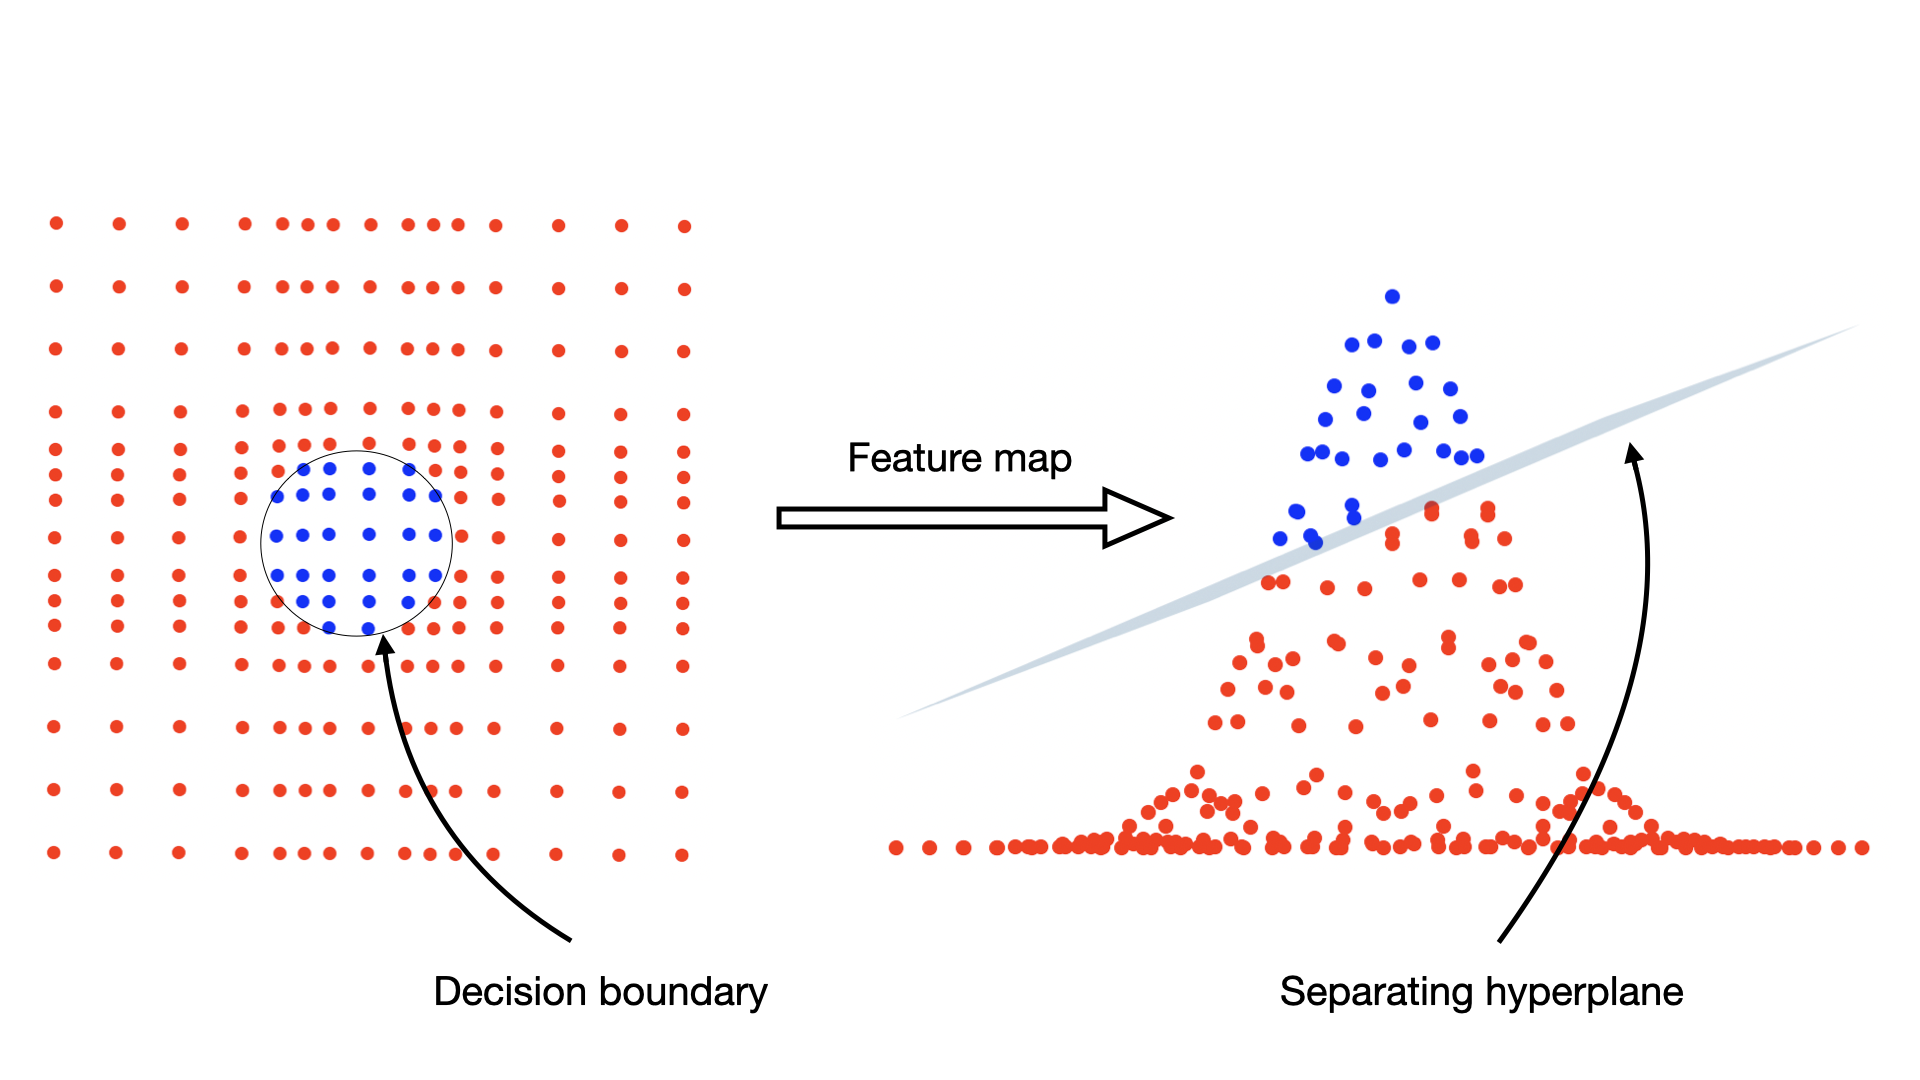
\includegraphics[width=0.98\textwidth]{assets/svm_comp_2.png}
		\caption*{SVM - Non-Linear Separation - Kernel Trick}
	\end{figure}
\end{frame}


\subsection{The Fusiform Gyrus}

\begin{frame}
\frametitle{The Fusiform Gyrus}
\begin{columns}
	\begin{column}{0.5\textwidth}
		\begin{itemize}
			\uncover<1->{\item Primarily located in\\the temporal lobe}
			\uncover<2->{\item Home to the Fusiform Face Area (\textit{FFA}) and the Parahippocampal Place Area (\textit{PPA}), partly}
			\uncover<3->{\item Category selectivity is more localized and stronger,\\based on literature}
		\end{itemize}
	\end{column}

	\begin{column}{0.49\textwidth}
		\only<1>{
			\begin{figure}
				\centering
				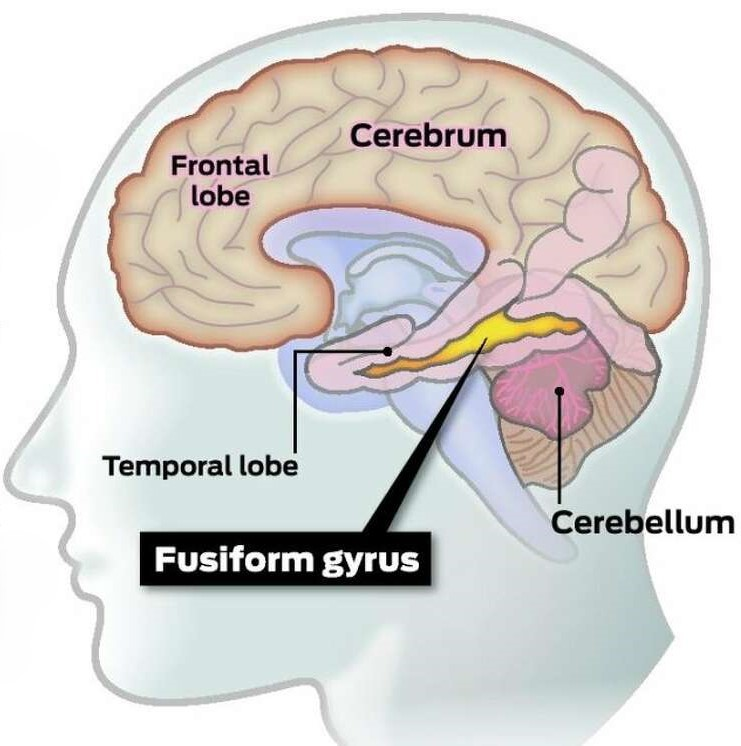
\includegraphics[width=0.98\textwidth]{assets/fusiform_gyrus.jpg}
				\caption*{The Fusiform Gyrus Location in the Human Brain (\textit{Saggital Plane})}
			\end{figure}
			}
		\only<2>{
			\begin{figure}
				\centering
				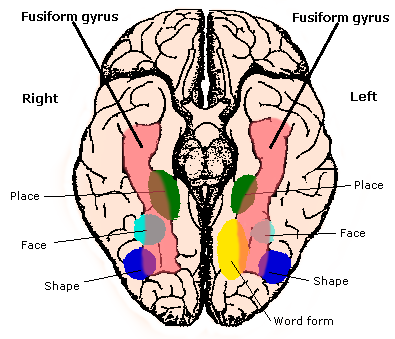
\includegraphics[width=0.98\textwidth]{assets/fusiform_gyrus_2.png}
				\caption*{The Fusiform Gyrus Location in the Human Brain (\textit{Horizontal Plane})}
			\end{figure}
			}
		\only<3>{
			\begin{figure}
			\centering
			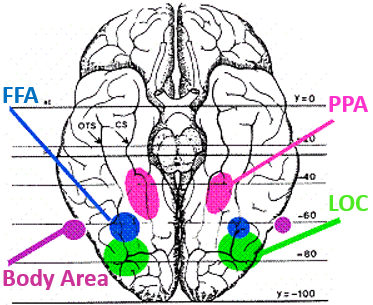
\includegraphics[width=0.98\textwidth]{assets/brain_areas.png}
			\caption*{Category-Specific Stimulus Information Processing Centers}
			\end{figure}
			}
	\end{column}
\end{columns}
\end{frame}


\subsection{Why fMRI?}
\begin{frame}
\frametitle{Why fMRI?}

    \begin{itemize}
        \uncover<1->{\item High spatial resolution (mm), ideal for studying localized functions}
        \uncover<2->{\item Whole brain coverage, highlighting interaction among regions}
        \uncover<3->{\item Measures BOLD signal, indirectly associated with neuronal activity}
        \uncover<4->{\item Low temporal resolution, allowing the study of longer-term brain processes (s), but potential problem for quick responses}
    \end{itemize}
\end{frame}